\documentclass{beamer}

\usepackage{pythonhighlight}

\usepackage{graphicx}
\usepackage[dutch]{babel}

\usepackage{amsmath}

\title{Self-avoiding walks}
\subtitle{in het hexagonale vlak}
\author{Thomas van Maaren}
\date{24 mei 2022}

%\usetheme{lucid}
\begin{document}
	\frame {
		\titlepage
	}
	\frame {
		\frametitle{Inhoud}
		\begin{itemize}
			\item Wat zijn self-avoiding walks?
			\item Toepassing van self-avoiding walks
			\item Lengte van self-avoiding walks
			\item Mogelijke self-avoiding walks
			\item Hongingraat
			\item Algoritme voor het bepalen van mogelijke walks
			\item Demonstratie algoritme (Turtle graphics)
			\item Ondergrenzen/bovengenzen
			\item Antwoord op de vraag
			\item Connective constant
		\end{itemize}
	}
	\frame{
		\frametitle{Wat zijn self-avoiding walks?}
		\begin{tabular}{c c}
			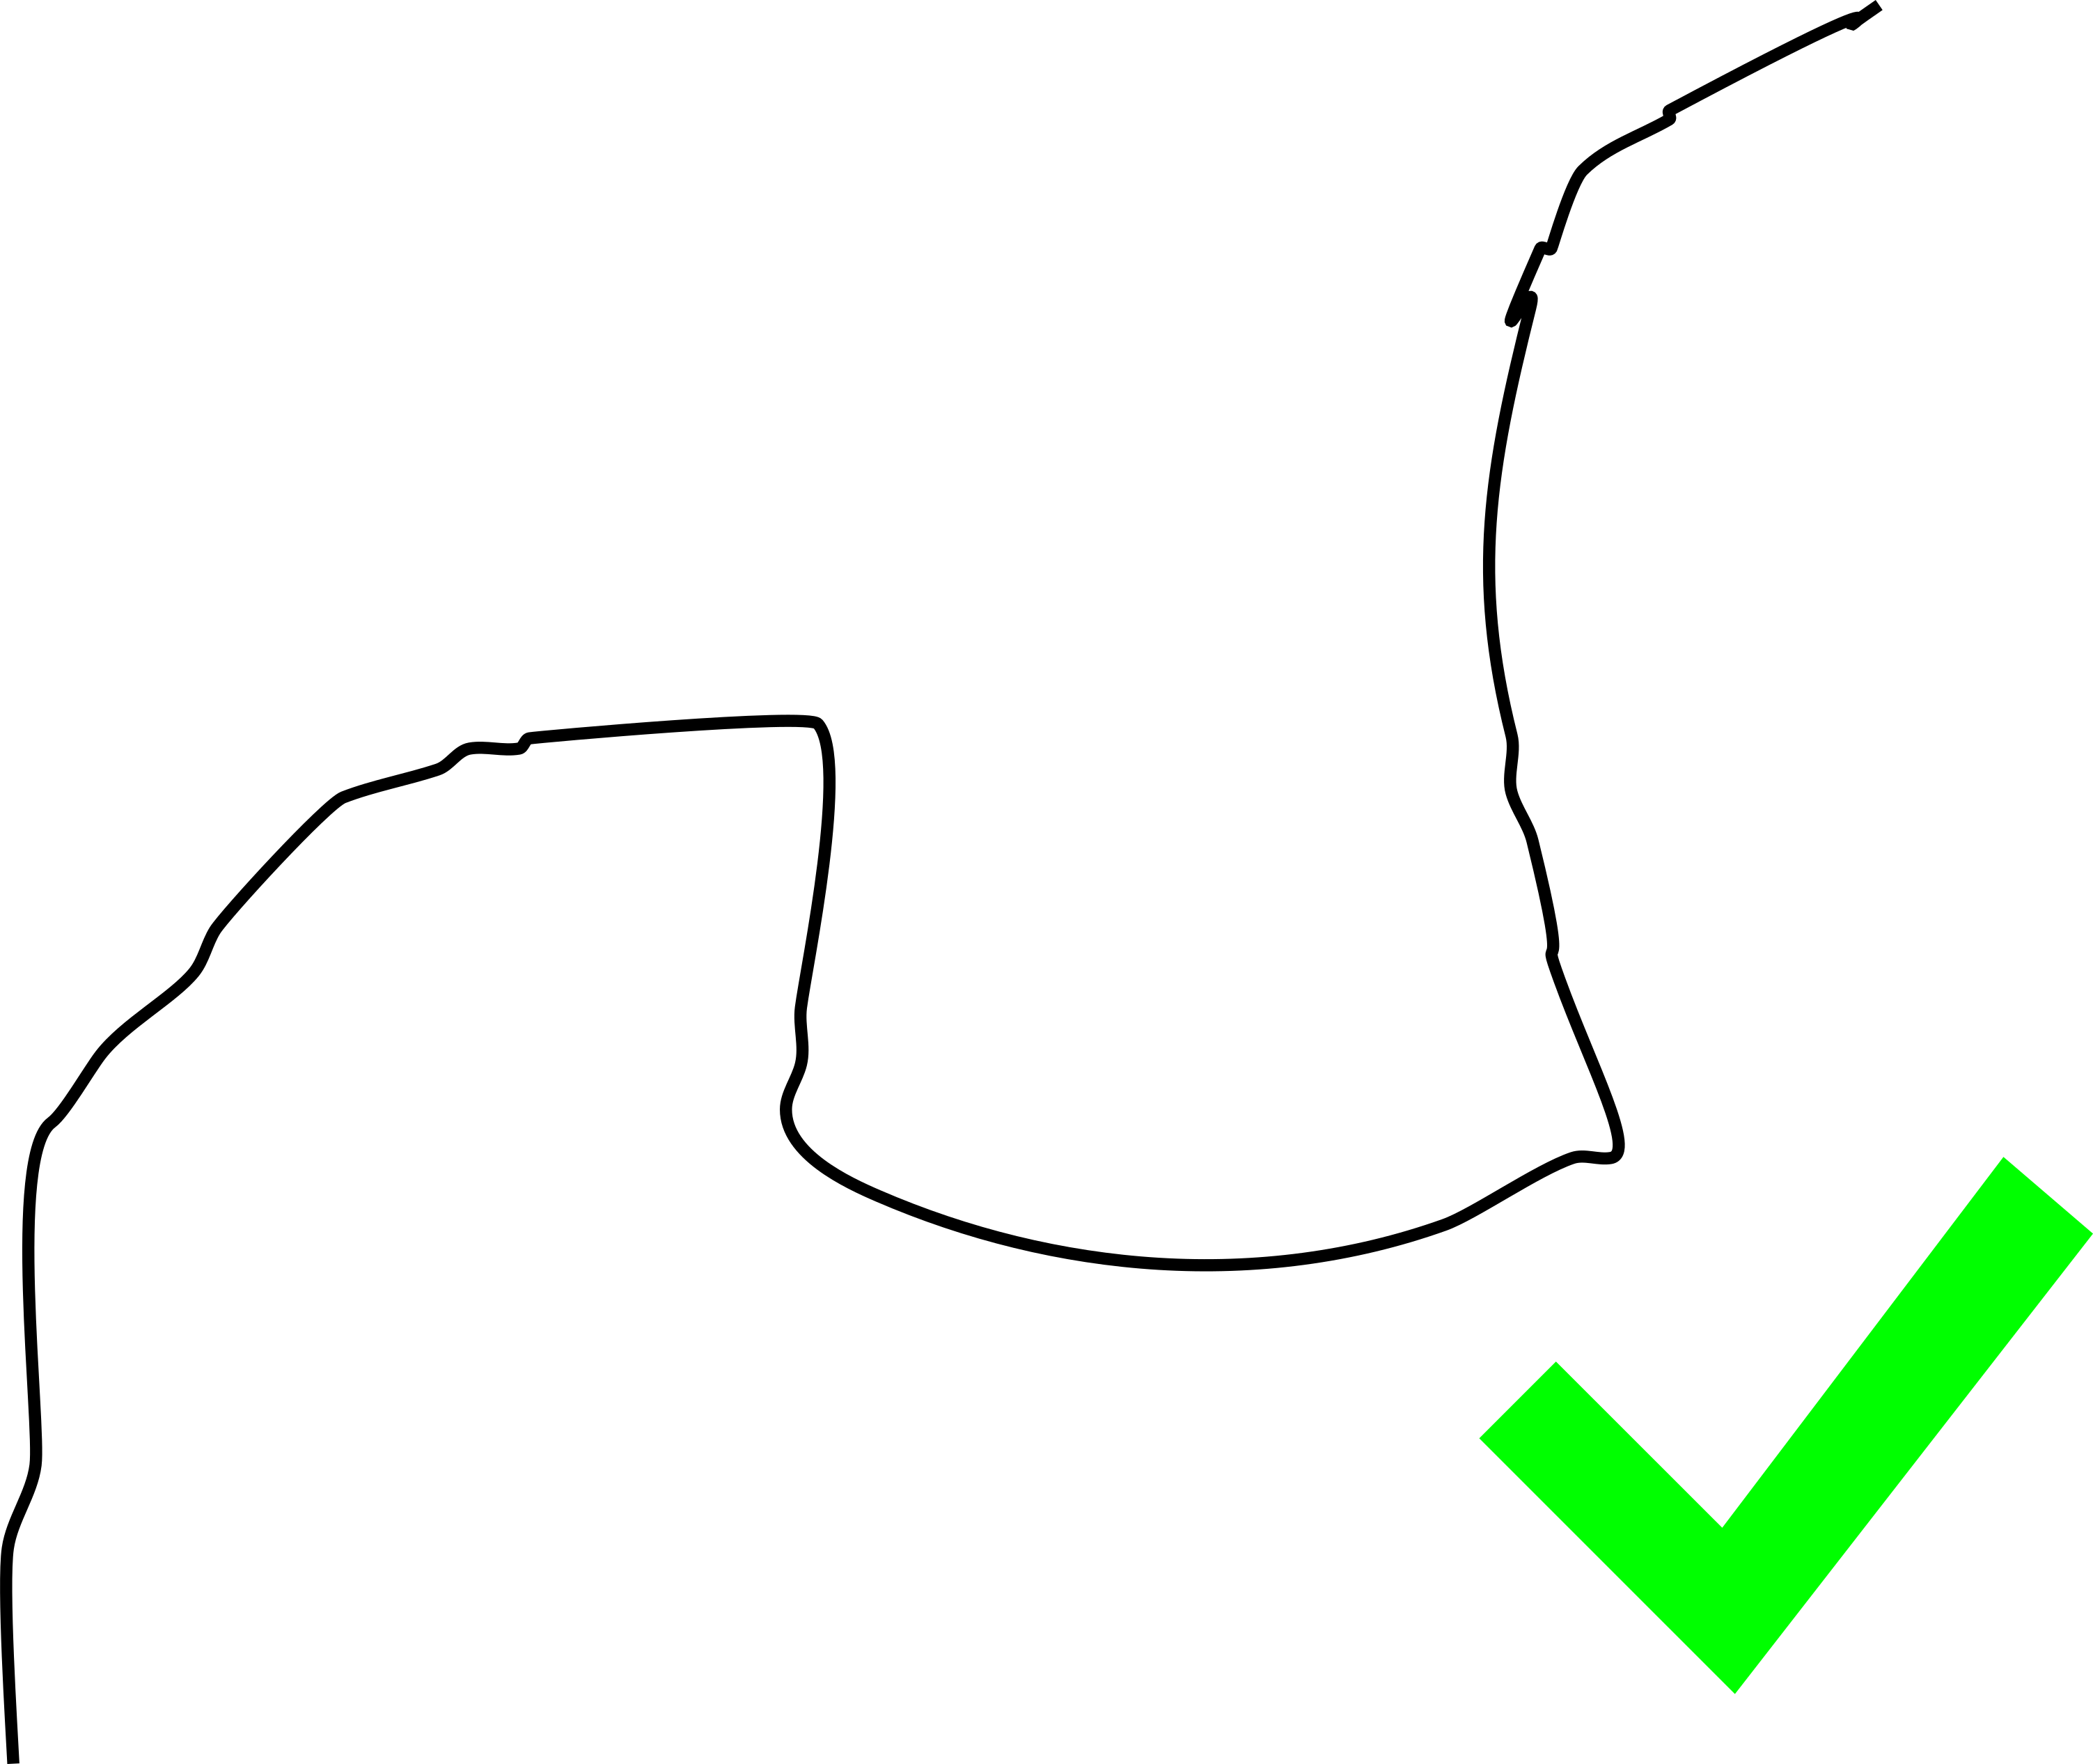
\includegraphics[width=0.5\textwidth]{Wel_een_avoiding_walk.png} 
			& 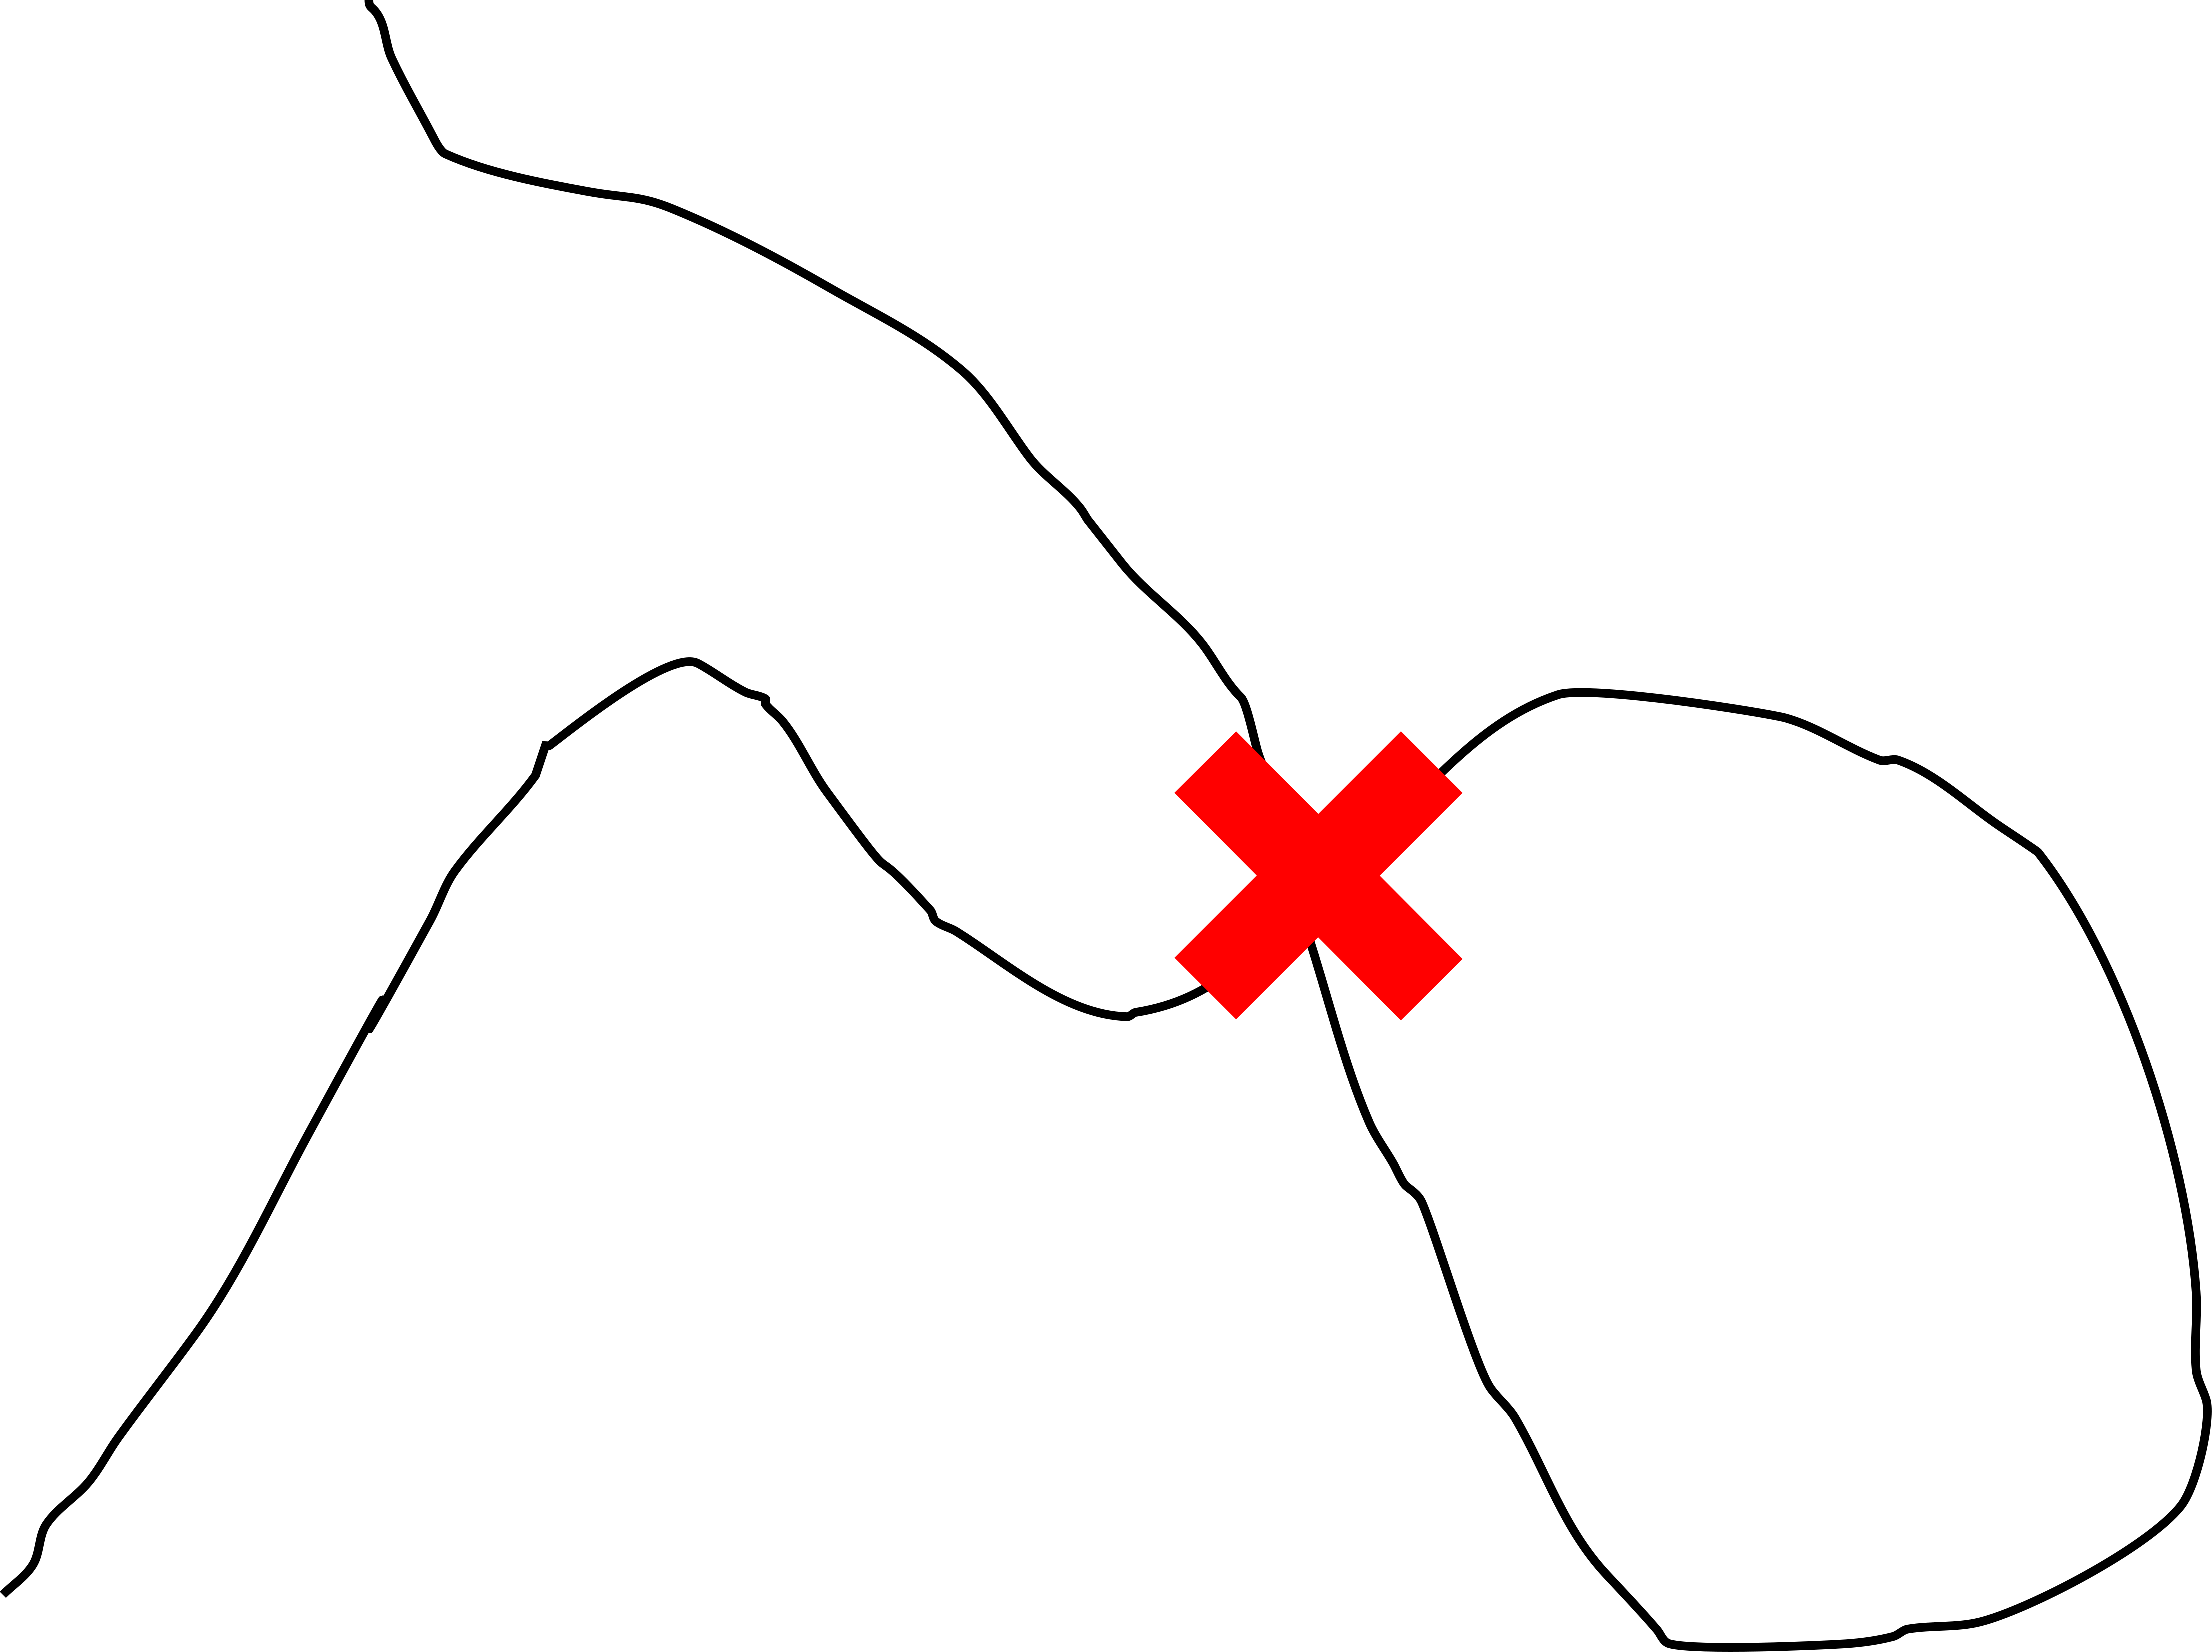
\includegraphics[width=0.5\textwidth]{geen_avoiding_walk.png}\\
			Wel een self-avoiding walk & Geen self-avoiding walk\\
		\end{tabular}
	}
	\frame{
		\frametitle{Toepassingen van self-avoiding walks}
		\begin{figure}
			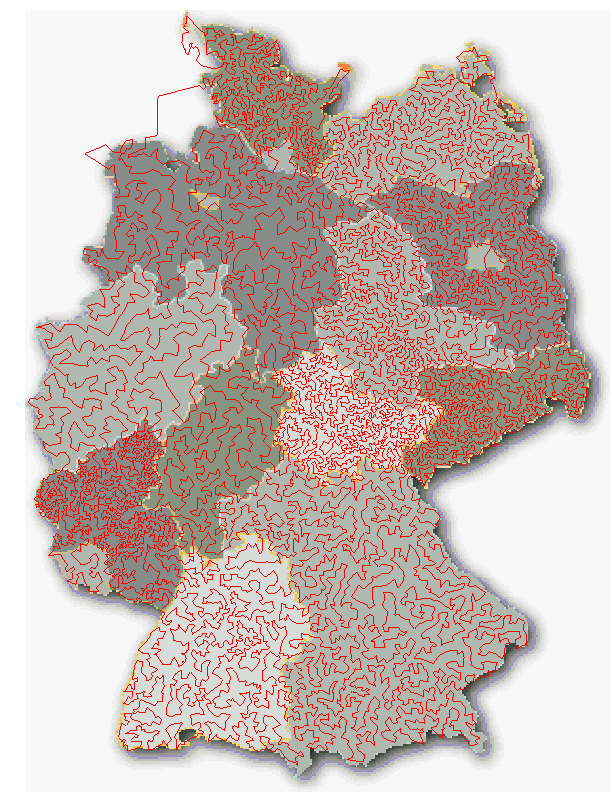
\includegraphics[height=0.75\textheight]{d15map_big.png}
			\caption{Optimale weg door 15112 duitse steden. Bron:University of Waterloo}
		\end{figure}
	}
	\frame{
		\frametitle{Lengte van een Avoiding walk}
		\begin{tabular}{c c}
			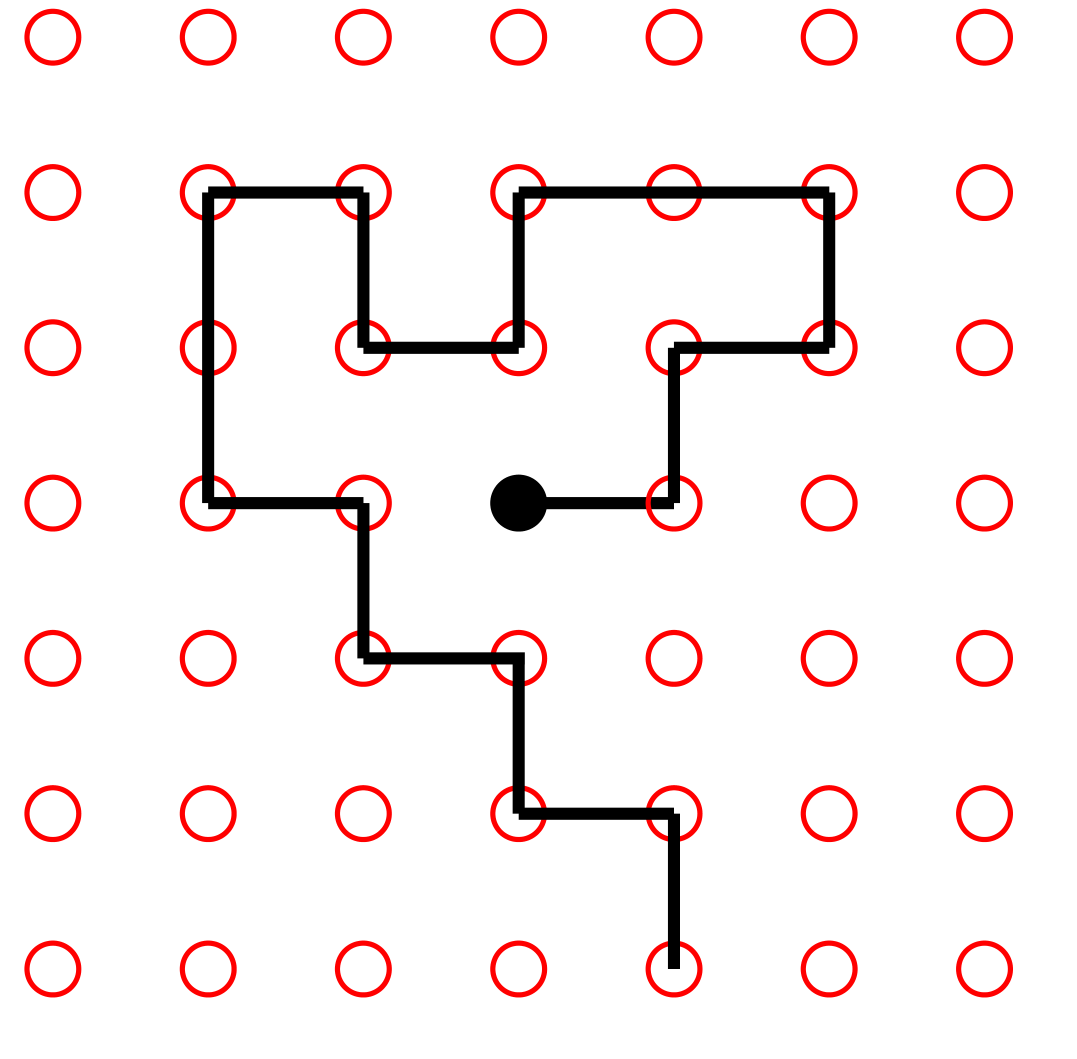
\includegraphics[width=0.5\textheight]{grid.png}&
			\includegraphics[width=0.5\textheight]{Hexagonale vlak.png}\\
			 Lengte 18 op een vierkant rooster & Lengte 13 op een honingraat\\
		\end{tabular}
	}
	\frame{
		\frametitle{Mogelijke self-avoiding walks}
		Zij $n\in \mathbb{N}$. Dan definieren $c_n$ als het aantal
		mogelijke self-avoiding walks met lengte $n$ die vanaf de oorsprong op een honingraat gemaakt
		kunnnen worden.

		\begin{itemize}
			\item  $c_1=3$
			\item  $c_2=3\cdot 2=6$
			\item  $c_3=3\cdot 2^2=12$
			\item  $c_4=3\cdot 2^3=24$
			\item  $c_5=3\cdot 2^4=48$
			\item  $c_6=3\cdot 2^5-6=96-6=90$
		\end{itemize}
	}
	\frame{
		\frametitle{Hongingraat}
		\begin{figure}
		\includegraphics[width=\textwidth]{honingraat_richtingen.png}
		\caption{Co\"ordinaten op een honingraat}
		\end{figure}
	}
	\frame{
		\frametitle{Algoritme voor het bepalen van mogelijke walks (1)}
		\inputpython{self-avoiding-walk.py}{1}{11}
	}
	\frame{
		\frametitle{Algoritme voor het bepalen van mogelijke walks (2)}
		\inputpython{self-avoiding-walk.py}{12}{22}
	}
	\frame{
		\frametitle{Demonstratie}
	}
	\frame{
		\frametitle{Bovengrenzen en ondergrenzen}
		We kunnen zeggen dat $c_n$ de volgende ondergrenzen en bovengrenzen heeft.
		$$\sqrt{2}^n\leq c_n \leq 3\cdot 2^n$$
		Aangezien we een pad op kunnen splitsen zien we ook dat
		$$c_{m+n}\leq c_mc_n$$
		\textbf{Vraag aan jullie:} Convegeert de rij $c_n^{\frac{1}{n}}$?
	}
	\frame{
		\frametitle{Antwoord op de vraag}
		Het convergeert wel. We zien eerst dat $\sqrt{2} \leq
		c^{\frac{1}{n}}$, dus heeft het een infimum die we noteren met
		$L$. Zij $\epsilon>0$. We weten dan dat er een $k\in
		\mathbb{N}$ zodat $c_k^{\frac{1}{k}}\leq L+\epsilon$. %Voor alle $n>k$ zien we
		dat $n=p_nk+q_n$ voor een $p_n,q_n\in \mathbb{N}$, waarbij 
		$0\leq q_n\leq p_n$. We zien nu dat 

		$$c_n^{1/n}=c_{p_nk+q_n}^{1/n}\leq (c_k^{p_n}c_{q_n})^{1/n}=(c_k^{\frac{1}{k}})^{\frac{p_nk}{n}}c_{q_n}^{\frac{1}{n}}$$

		We zien dat $\lim_{n\to \infty} \frac{p_n}{n}=1$ en $\lim_{n\to \infty}\frac{1}{n}=0$, dus 

		$$
		\lim_{n \to \infty} (c_k^{\frac{1}{k}})^{\frac{p_nk}{n}}c_{q_n}^{\frac{1}{n}}
		=(c_k^{\frac{1}{k}})^1c_{q_n}^0
		=c_k^{\frac{1}{k}}
		$$

		Dus is er een $N\in \mathbb{N}$ waar voor alle $n>N$ geldt $(c_k^{\frac{1}{k}})^{\frac{p_nk}{n}}c_{q_n}^{\frac{1}{n}}\leq L+\epsilon$. Dus voor alle $n>N$ geldt dan ook dat $c_n^{\frac{1}{n}}\leq L+\epsilon$

		%en dus $L\leq \lim_{n\to \infty}c_n^{1/n}\leq c^{\frac{1}{k}}_k\leq L+\epsilon$. Dus $\lim_{n\to \infty}c_n^{1/n}=L$.
	}

	\frame{
		\frametitle{Connective constant}
		De connective constant is $lim_{n\to \infty} c_n^{\frac{1}{n}}$. Voor een bijenraad is dit

		$$\sqrt{2+\sqrt{2}}\approx 1.8478$$

		Voor andere roosters is dit ongeveer

		\begin{itemize}
			\item Driehoeksrooster: 4.15079
			\item Vierkantrooster: 2.6381585
		\end{itemize}
		
	}
\end{document}
